\section{\LangOO, The underlying programming language } %-- a small  object oriented programming language}

\subsection{\LangOO syntax runtime configurations}
\label{sub:Loo} 
 \LangOO  is a {small}, imperative, sequential,  class based, typed, object-oriented language, % whose fields are private to the class where they are defined, 
 with private fields, private or public methods, unforgeable addresses, and no ambient authority (no static methods, no address manipulation).
 It has a simple concept of module, and module private fields and methods, described in Sect. \ref{sect:execution}.
 %, and whose   methods may be private (callable only form internal objects), or public (callable from all objects).
The complete definition of \LangOO  {can be found in the appendices  \cite{necessityFull}}, and is  similar to   OOPSLA-22.\footnoteSD{any differences?}

A \LangOO state, $\sigma$,  consists of a  heap $\chi$, and a   stack $\psi$. A stack is is a sequence of frames, $\phi$.
A frame consists of local variable map, and a continuation, \ie a sequence of statements to be executed.

 
\paragraph{Notation} We adopt the following, un-surprising, notation:
\begin{itemize}
\item
$\alpha$, $\alpha'$, $\alpha_1$, ... are addresses,   $x$, $x'$, $x_1$, ..., $y$, ... $z$, ... are variables, and $\va$, $\va'$ ... are either addresses or variables, we call these \emph{\atoms}.
%\item
%Assertions, $A$, and simple expression, $e$, are described in Def. \ref{def:assert:syntax}. They support  the usual connectives as well as connectives about protection. An assertion may  expressions, $e$. These may contain variables, addresses, field look-ups, and ghost-field look-ups, but \emph{not} method calls; the latter may appear in assertions, and \emph{not} in code, while the former may \emph{not}.
\item
$\alpha \in \sigma$ means that $\alpha$ is defined in the heap of $\sigma$, and $x\in \sigma$ means that $x$ is defined in the top frame of $\sigma$.
`%, and $x\in A$ means that $x$ appears free $A$. 
Conversely, % $\alpha$ is fresh, resp.$x$ is fresh in $\sigma$   in $\sigma$ means that 
 $\alpha\notin\sigma$, and. $x\notin\sigma$ %, and $\va \notin A$ h
 ave the obvious meaning.
\item
$\interpret{\sigma}{\alpha}$  is $\alpha$; and $\interpret{\sigma}{x}$  is the value to which  $x$  is mapped in the top-most frame of $\sigma$'s stack; 
and $\interpret{\sigma}{e.f}$ looks up in $\sigma$'s heap the value of $f$ for the object  $\interpret{\sigma}{e}$.
Note that $\interpret{\sigma}{e}$ is not defined when $e$ contains a method call or a ghost field.
\item The substitution  $\sigma[x \mapsto \alpha]$ is applied to the top frame of $\sigma$, and $\sigma[\overline{x \mapsto \alpha}]$ % applies the substitutions $\overline{x \mapsto \alpha}$ to the top frame.
has the expected meaning.
\end{itemize}

  
\newcommand{\Mext}{M_{extl}}
\newcommand{\Mint}{M\_{intl}}
\newcommand{\Mtwo}{\overline{M}}
  
\subsection{\LangOO Execution, and internal/external modules }
\label{sect:execution}

%Central to our work is the distriction between the 
 \LangOO execution it is a small steps operational semantics of the shape $\leadstoOrig  {\Mtwo} {\sigma}   {\sigma'}$.
 It takes place \red{in the context of one or more modules, $\Mtwo$}.
 A module,  $M$, is a mappings from class names to class definitions. 
   
The semantics enforces dynamically a simple form of package-wide privacy: 
Fields may be read or written only if the class of the object whose field is being read or written, and the class of the object which is reading of writing belong to the same module.
Private methods may be called only if the class of the receiver (the object whose method is being called), and the class of the caller (the object which is calling) belong to the same module.
Public methods may always be called.

The semantics is as un-surprising in  all remaining aspects  :  
In $\sigma$, the  top frame's continuation contains the statement to be  executed next.  
 A statement may assign to variables, allocate a new object, 
perform field reads and writes on objects,  or
 call methods on those objects. 
When a method is called, a new frame is pushed on to the stack; this frame  maps \prg{this} and the formal parameters to  the values for the receiver and other arguments, and the continuation to the body of the method.  When the continuation is ground\footnoteSD{TODO check and define}, the frame is popped and the value from the last frame's continuation is entered into the appropriate part in the caller's continuation. 
%In other aspects, the semantics is un-surprisring.%we return from that call, its frame is  popped, and execution continues in the context of the calling method.
%The relation $\leadstoOrigStar  {\Mtwo} {\_}   {\_}$  is the reflexive, transitive closure of $\leadstoOrig  {\Mtwo} {\_}   {\_}$ .


{Fig. \ref{fig:UpSemantics} illustrates  such  execution steps:  black disks indicate states;
 horizontal $\leadsto$-arrows denote   steps  within the same  call; upwards arrows denote  method calls;
 %(pushing a new frame onto the stack);  
 downwards arrows denote method returns. % (popping the top of the stack). 
 Here,   $\leadstoOrig {\Mtwo}{\sigma_8}   {\sigma_9} $ is a step within the same call, $\leadstoOrig {\Mtwo}{\sigma_9}   {\sigma_{10}} $ is a method call   
with $\leadstoOrig {\Mtwo}{\sigma_{12}}   {\sigma_{13}} $ %is a method return  (from the call to $m_a$), 
the corresponding return. 
\red{Note that  $\leadstoOrigStar  {\Mtwo} {\sigma}   {\sigma'}$ may involve  any number of  calls or returns: 
 $\leadstoOrigStar  {\Mtwo} {\sigma_8}   {\sigma_{12}}$ involves one call and no return,
while $\leadstoOrigStar  {\Mtwo} {\sigma_{10}}   {\sigma_{15}}$,   involves no calls and two returns.
% In section \ref{sect:bounded}, we will define a derived relation, called bounded execution, where the number of returns may not exceed the number of calls.
}
} 

\begin{figure}[htb]
\begin{tabular}{|c|}
 \hline %  \\ -- this added one vertical space
\resizebox{7cm}{!}{
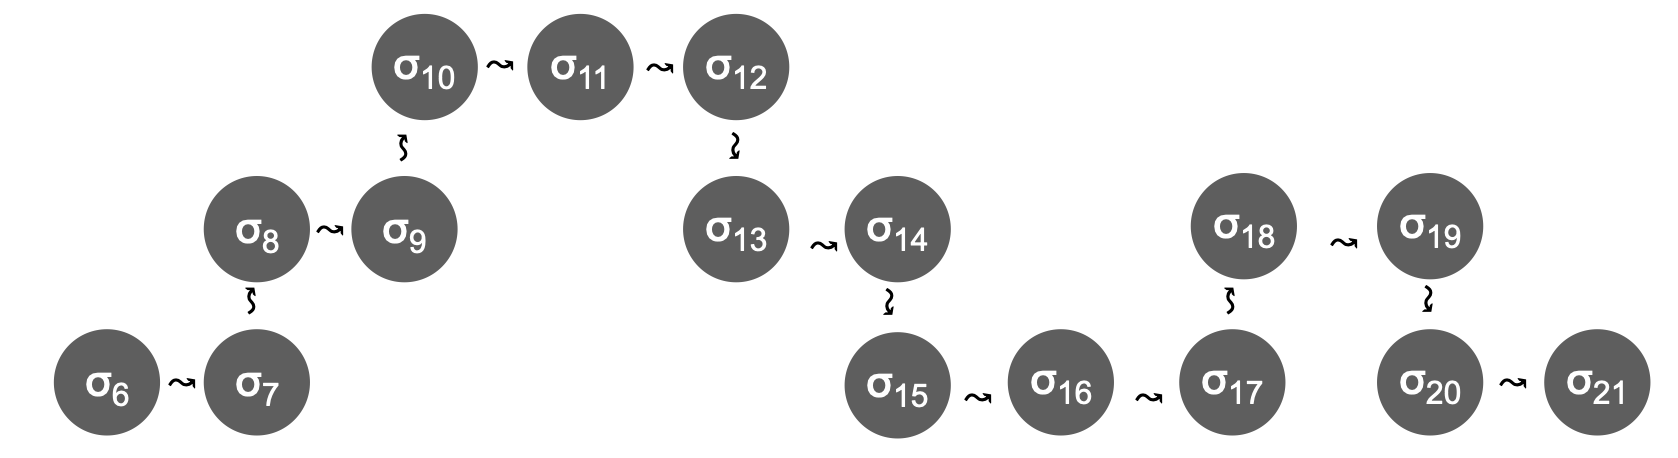
\includegraphics[width=\linewidth]{diagrams/bounded.png}
} 
 \\
\hline
\begin{tabular}{lclclclcl}
 $\leadstoOrig  {\Mtwo} {\sigma_8}    {\sigma_9} $  & &  $\leadstoOrig  {\Mtwo} {\sigma_9}    {\sigma_{10}} $ &  &
$\leadstoOrig  {\Mtwo} {\sigma_{12}}   {\sigma_{13}} $ & &  $\leadstoOrig  {\Mtwo} {\sigma_{13}}    {\sigma_{14}} $  &  & $\leadstoOrig {\Mtwo}{\sigma_{14}}   {\sigma_{15}} $
\\
\hline
$\leadstoOrigStar  {\Mtwo} {\sigma_8}   {\sigma_{12}}$ & & \ & & \ & & $\leadstoOrigStar  {\Mtwo} {\sigma_{10}}   {\sigma_{15}}$
\\
\hline
%%Bound
%\ \ \  $\leadstoBounded  {\Mtwo} {\sigma_{12}} {\sigma_8}  {\sigma_{13}} $ \ \ \ \ \ \ \  $\leadstoBounded  {\Mtwo} {\sigma_{13}}  {\sigma_{8}}  {\sigma_{14}} $ 
%\\ 
%%ORIG
%$\leadstoOrig {\Mtwo}{\sigma_{14}}   {\sigma_{15}} $  \ \ \ \ \ \ \  
%\ \ \ \ \ \ \  \ \ \ & \ \ \ 
%%BOUND
%$\notLeadstoBounded  {\Mtwo} {\sigma_{14}} {\sigma_8}  {\sigma_{15}} $
%\end{tabular}
%\\
%\hline

%\begin{tabular}{l|l}
%\ \ \ \ \ \ \  \ \ \ \ \ \ \  \ \ \ \ \ Execution \ \ \ \  &  \ \ \ \ \ \ \  \ \ \ \ \ \ \   \ \ \ \ \  Bounded Execution \ \ \ \  \\
%\hline % \\
% $\leadstoOrig  {\Mtwo} {\sigma_8}    {\sigma_9} $ \ \ \ \ \ \ \ \  \ $\leadstoOrig  {\Mtwo} {\sigma_9}    {\sigma_{10}} $ & 
%%Bound
%\ \ \  $\leadstoBounded  {\Mtwo} {\sigma_8} {\sigma_8}  {\sigma_9} $ \ \ \ \ \ \ \ \  \ $\leadstoBounded  {\Mtwo} {\sigma_9} {\sigma_8}  {\sigma_{10}} $
%\\
%$\leadstoOrig  {\Mtwo} {\sigma_{12}}   {\sigma_{13}} $ \ \ \ \ \ \ \  $\leadstoOrig  {\Mtwo} {\sigma_{13}}    {\sigma_{14}} $  & 
%%Bound
%\ \ \  $\leadstoBounded  {\Mtwo} {\sigma_{12}} {\sigma_8}  {\sigma_{13}} $ \ \ \ \ \ \ \  $\leadstoBounded  {\Mtwo} {\sigma_{13}}  {\sigma_{8}}  {\sigma_{14}} $ 
%\\ 
%%ORIG
%$\leadstoOrig {\Mtwo}{\sigma_{14}}   {\sigma_{15}} $  \ \ \ \ \ \ \  
%\ \ \ \ \ \ \  \ \ \ & \ \ \ 
%%BOUND
%$\notLeadstoBounded  {\Mtwo} {\sigma_{14}} {\sigma_8}  {\sigma_{15}} $
\end{tabular}
\\
\hline
\end{tabular}
   \caption{Illustrating   $\leadstoOrig  {\Mtwo} {\sigma}    {\sigma'}$
    }
   \label{fig:UpSemantics}
 \end{figure}
 
 
 
%\sdN{Note that $\leadstoOrig {\Mtwo}{\sigma_{8}}   {\sigma_{9}} $ and $\leadstoOrig {\Mtwo}{\sigma_{13}}   {\sigma_{14}} $ are steps within the same call, but 
%$\leadstoOrig {\Mtwo}{\sigma_{14}}   {\sigma_{15}} $ and $\leadstoOrig {\Mtwo}{\sigma_{17}}   {\sigma_{18}} $ are not. %steps within the same call,
%% even though all four states ($\sigma_{13}$, $\sigma_{14}$, $\sigma_{17}$, and $\sigma_{18}$), have the same number of frames on their stack.
%We want a semantics to reflect whether execution steps happen within the bounds of certain call. For this, we define \emph{bounded execution}, 
%$\leadstoBounded {\Mtwo} {\sigma} {\sigma''} {\sigma'}$ 
%which are execution steps which lead from $\sigma$ to $\sigma'$ while not popping  $\sigma''$-s top frame.
%This will be defined in Section \ref{sect:bounded}.
%}

\subsection*{Applicability} 
While our work is based on the particular language  \LangOO , % a simple, imperative, typed, object oriented  language with unforgeable addresses and private fields, we believe that % our approach
we believe that it is applicable to several programming paradigms, and  that   unforgeability and privacy
 can be replaced  by lower level mechanisms such as capability machines \cite{vanproving,davis2019cheriabi}.


\section{From \LangOO to \AssertLang}

\sdN{In order to give semantics of our assertions language, \AssertLang, we need to build three auxiliary concepts on  top of  \LangOO: bounded execution, locally  reachable objects, and pushing of frames.}


\subsection{Bounded Execution}
\label{sect:bounded}

\sdN{The semantics from the earlier section allows arbitrary method calls and returns. % pushing and poping frames from the stack in arbitrary fashion. 
In particular it is possible to start with a state $\sigma$ and perform more returns than calls --
% after a number of execution steps to reach a state $\sigma'$ with fewer frames on its stack -- 
cf . $\leadstoOrigStar  {\Mtwo} {\sigma_{8}}   {\sigma_{15}}$ from earlier.
However,  from $\sigma_8$'s viewpoint the future only incudes states which are being visited as a result of  $\sigma_8$'s top continuation; that is, it includes the states $\sigma_9$, $\sigma_{10}$, $\sigma_{11}$, $\sigma_{12}$, $\sigma_{13}$, and $\sigma_{13}$, but \emph{not} $\sigma_{15}$, or $\sigma_{18}$, etc.
% since $\sigma$'s top frame will have been popped before we reach $\sigma'$. 
We therefore define another version of execution which is from the viewpoint of an original state, $\sigma_o$, and which  is ``bounded'' so as not to ever pop the top grame of   $\sigma_o$}


{
\begin{definition}[Bounded Execution]
\label{def:shallow:term}
We define the relation  $\leadstoBounded {\Mtwo} {\sigma_1} {\sigma_o} {\sigma_2}$ 

\begin{itemize}
\item
 $\leadstoBounded {\Mtwo} {\sigma} {\sigma_o}  {\sigma'}$ \ \ \ iff \ \ \  $\leadstoOrig {\Mtwo} {\sigma} {\sigma'}$\\
$\strut  \hspace{3.6cm} \wedge $\\
$\strut  \hspace{3.1cm}\ \    \exists \phi,\psi, \phi_1, \phi2.[ \ \sigma_o = (\phi\cdot\psi,\_) \ \wedge \ \sigma = (\psi_1\cdot \psi, \_)
\ \wedge\ \sigma' = (\psi_2\cdot \psi, \_)\ ] $ 
\item
 $\leadstoBoundedStar {\Mtwo}  {\_}  {\sigma_o} {\_}$\ \  is the reflexive, transitive closure of $\leadstoBounded {\Mtwo}  {\_}  {\sigma_o} {\_}$.
\end{itemize}
\end{definition}
}
 
 \sdN{Continuing our discussion of Fig. \ref{fig:UpSemantics}, notice that $\leadstoOrig {\Mtwo} {\sigma_{14}}  {\sigma_{15}}$ 
 but    $\notLeadstoBounded  {\Mtwo}  {\sigma_{14}} {\sigma_8} {\sigma_{15}}$:  this step would pop  $\sigma_8$'s
 top frame. 
Therefore, 
 $\leadstoOrigStar {\Mtwo} {\sigma_8}  {\sigma_{15}}$ 
 but  $\notLeadstoBoundedStar {\Mtwo} {\sigma_8} {\sigma_8} {\sigma_{15}}$, and also
  $\leadstoOrigStar {\Mtwo} {\sigma_8}  {\sigma_{18}}$ 
 but  $\notLeadstoBoundedStar {\Mtwo} {\sigma_8} {\sigma_8} {\sigma_{18}}$  -- the latter reflects that $\sigma_8$ and $\sigma_{18}$ belong to different calls. 
}

\begin{figure}[htb]
\begin{tabular}{|c|}
 \hline %  \\ -- this added one vertical space
\resizebox{7cm}{!}{
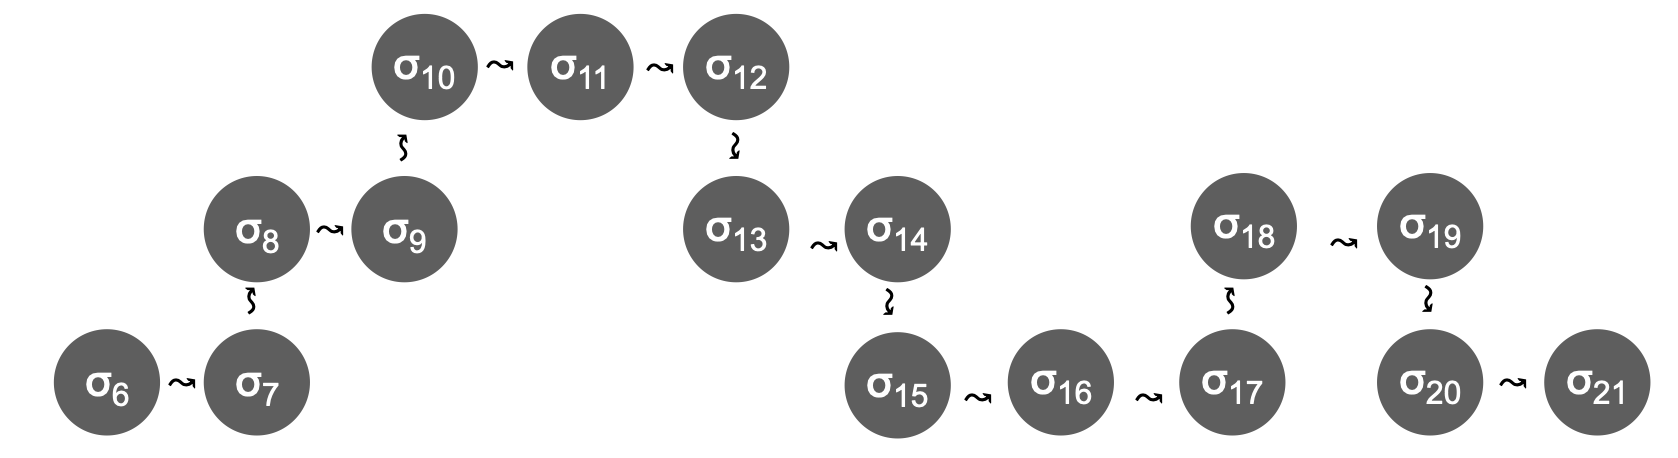
\includegraphics[width=\linewidth]{diagrams/bounded.png}
} 
 \\
\hline
\begin{tabular}{lclclclcl}
 $\leadstoBounded  {\Mtwo} {\sigma_{12}} {\sigma_8}  {\sigma_{13}} $  & &   $\leadstoBounded  {\Mtwo} {\sigma_{13}}  {\sigma_{8}}  {\sigma_{14}} $ &  &
$\notLeadstoBounded  {\Mtwo} {\sigma_{14}} {\sigma_8}  {\sigma_{15}} $ & &  
\\
%%Bound
%\ \ \  $\leadstoBounded  {\Mtwo} {\sigma_{12}} {\sigma_8}  {\sigma_{13}} $ \ \ \ \ \ \ \  $\leadstoBounded  {\Mtwo} {\sigma_{13}}  {\sigma_{8}}  {\sigma_{14}} $ 
%\\ 
%%ORIG
%$\leadstoOrig {\Mtwo}{\sigma_{14}}   {\sigma_{15}} $  \ \ \ \ \ \ \  
%\ \ \ \ \ \ \  \ \ \ & \ \ \ 
%%BOUND
%$\notLeadstoBounded  {\Mtwo} {\sigma_{14}} {\sigma_8}  {\sigma_{15}} $
%\end{tabular}
%\\
%\hline

%\begin{tabular}{l|l}
%\ \ \ \ \ \ \  \ \ \ \ \ \ \  \ \ \ \ \ Execution \ \ \ \  &  \ \ \ \ \ \ \  \ \ \ \ \ \ \   \ \ \ \ \  Bounded Execution \ \ \ \  \\
%\hline % \\
% $\leadstoOrig  {\Mtwo} {\sigma_8}    {\sigma_9} $ \ \ \ \ \ \ \ \  \ $\leadstoOrig  {\Mtwo} {\sigma_9}    {\sigma_{10}} $ & 
%%Bound
%\ \ \  $\leadstoBounded  {\Mtwo} {\sigma_8} {\sigma_8}  {\sigma_9} $ \ \ \ \ \ \ \ \  \ $\leadstoBounded  {\Mtwo} {\sigma_9} {\sigma_8}  {\sigma_{10}} $
%\\
%$\leadstoOrig  {\Mtwo} {\sigma_{12}}   {\sigma_{13}} $ \ \ \ \ \ \ \  $\leadstoOrig  {\Mtwo} {\sigma_{13}}    {\sigma_{14}} $  & 
%%Bound
%\\ 
%%ORIG
%$\leadstoOrig {\Mtwo}{\sigma_{14}}   {\sigma_{15}} $  \ \ \ \ \ \ \  
%\ \ \ \ \ \ \  \ \ \ & \ \ \ 
%%BOUND
%$\notLeadstoBounded  {\Mtwo} {\sigma_{14}} {\sigma_8}  {\sigma_{15}} $
\end{tabular}
\\
\hline
\end{tabular}
   \caption{Illustrating   $\leadstoBounded  {\Mtwo} {\sigma_o} {\sigma}  {\sigma'}$
    }
   \label{fig:UpSemantics}
 \end{figure}
\subsection{Pushing Frames}


\red{Since one of the aims of the current work is to reason abourt external calls, the point at which a method is called or returned from is of particular importance. 
We introduce the
% We also adopt the following, less widespread, notations
% \begin{itemize}
% probably not needed, or at most needed only in soundness section.
% \item The substitution $A[\sigma]$ replaces in $A$ all its free variables, $\overline x$, by their values,  $\overline{\interpret{\sigma}{x}}$.
% \item 
%$C\in M$ means that class $C$ is in the domain of module $M$. 
% \item
the symbol $\pushSymbol$ to describes the result of pushing a new frame on the stack: $ \PushS  {\alpha} {\sigma} $ is  the set of states obtained by pushing onto the stack of $\sigma$ a new frame with some continuation  and a local variable map with domain same as the number of elements $\overline \alpha$ and range  $\overline \alpha$, while leaving the heap unmodified. If $\sigma$'s continuation was a method call with receiver and arguments $\overline \alpha$, then  $ \PushS   {\alpha} {\sigma}$ describes all possible direct successor states of $\sigma$. The elements of $ \PushS  {\alpha} {\sigma} $ only differ in the identifiers in the local variable map of the top frame. 
}
%\item

%\end{itemize}

\begin{definition}
\label{def:push:frame}
Given a state $\sigma$, addresses $\overline \alpha$, and variables or addresses $\overline \va$, we define
\begin{itemize}
\item
$ \PushS  {\alpha} {\sigma} \ =\ \{ \ \sigma' \ \mid\ \sigma=(\psi, \chi)\  \wedge\  (\phi\cdot \psi, \chi) \ \wedge\ rng(\phi)=\overline \alpha \ \ \mbox{ for some } \phi, \psi, \chi \ \}$
\item
\sdN{$ \PushS  {\va}  {\sigma}$ is short for  $ \PushS  {\interpret {\sigma} {\va}} {\sigma} $.}
\end{itemize}
\end{definition}

 \sdN{Consider Fig. \ref{fig:UpSemantics} again: $\sigma_8\in   \PushS  {\alpha} {\sigma_7}$ for some $\overline \alpha$, and 
 $\sigma_{14}\in\PushS  {\alpha'} {\sigma_{15}}$ for some $\overline \alpha'$. Namely, $\sigma_8$ is the fist state right after calling a method with receiver and
 arguments $\overline \alpha$ and $\sigma_{14}$ is the last state before returning from that method call back to $\sigma_{15}$.
Note that $\overline \alpha$ may differ from $\overline \alpha'$, because between $\sigma_8$ and $\sigma_{15}$ there may 
have been assignments to local variables -- only the receiver will have remained the same.
Similarly, 
 $\sigma_{10}\in\PushS  {\alpha''} {\sigma_9}$ for some $\overline \alpha''$, and  $\sigma_{12}\in\PushS  {\alpha'''} {\sigma_13}$ for some $\overline \alpha'''$, etc.
}


  \subsection{{Reachable  Objects}}

\red{A central concept to our work is object \emph{protection}, which we will define in   Sect. \ref{sect:protect}: It requires that no externa object which is 
reachable from the top frame  can have unmitigated access to that object.}
%
%{The  \SpecLang  specifications support universal quantification over  objects; such specifications 
%are applicable  to all objects in the heap witch, are however, either locally reachable (i.e. there is in the heap a path from the an 
%object on the top frame to the particular object), or globally reachable (i.e. there is in the heap a path from the an 
%object on some frame to the particular object.)
%%In this section  we will formally define these concepts.}\footnoteSD{TODO we need a better motivation for these concepts.}
%
An object $\alpha$ is  locally reachable, $ \LRelevant \alpha \sigma $, if it is reachable from the top frame on the stack of $\sigma$,
and it is globally reachable, $\GRelevant \alpha \sigma$, if it is reachable from from any  frame on the stack of $\sigma$.
 
\begin{definition} We define 
\begin{itemize}
\item
$ \LRelevant \alpha \sigma $ \ \ iff\ \  
$\exists \phi.[\ \sigma=(\phi\cdot\_, \_)$ and $\Relevant \alpha \phi \sigma\ ]$. % for some $\phi$
\item
$\GRelevant \alpha \sigma$  \ \ iff\ \  
$\exists \phi.[\ \sigma=(\_\cdot\phi\cdot\_, \_)$ and $\Relevant \alpha \phi \sigma\ ]$. % for some $\phi$
\end{itemize}
where\\
$\strut\ \ \ \  \ \ \ \ \ \ \Relevant \alpha \phi \sigma $  \ \ \ \ \ \ \ iff\ \  
$\exists n\in \mathbb{N}.\exists \prg{f}_1,... \prg{f}_n.\exists \prg{x}.[ \ \interpret{\sigma}{\phi(x).\prg{f}_1.....\prg{f}_n} = \alpha \ \ ]$.

\end{definition}

 \begin{figure}[htb]
\begin{tabular}{|c|c|c|}
\hline \\
\resizebox{3.5cm}{!}{
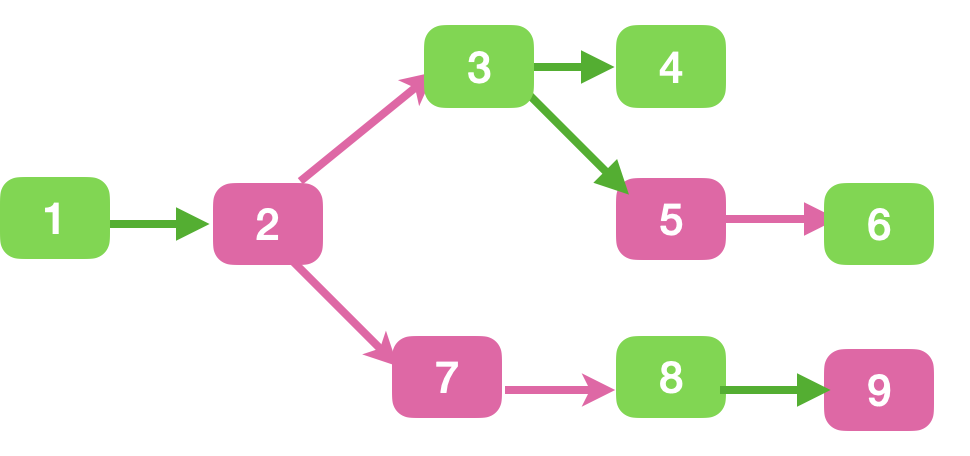
\includegraphics[width=\linewidth]{diagrams/heap.png}
} 
&
\resizebox{5cm}{!}{
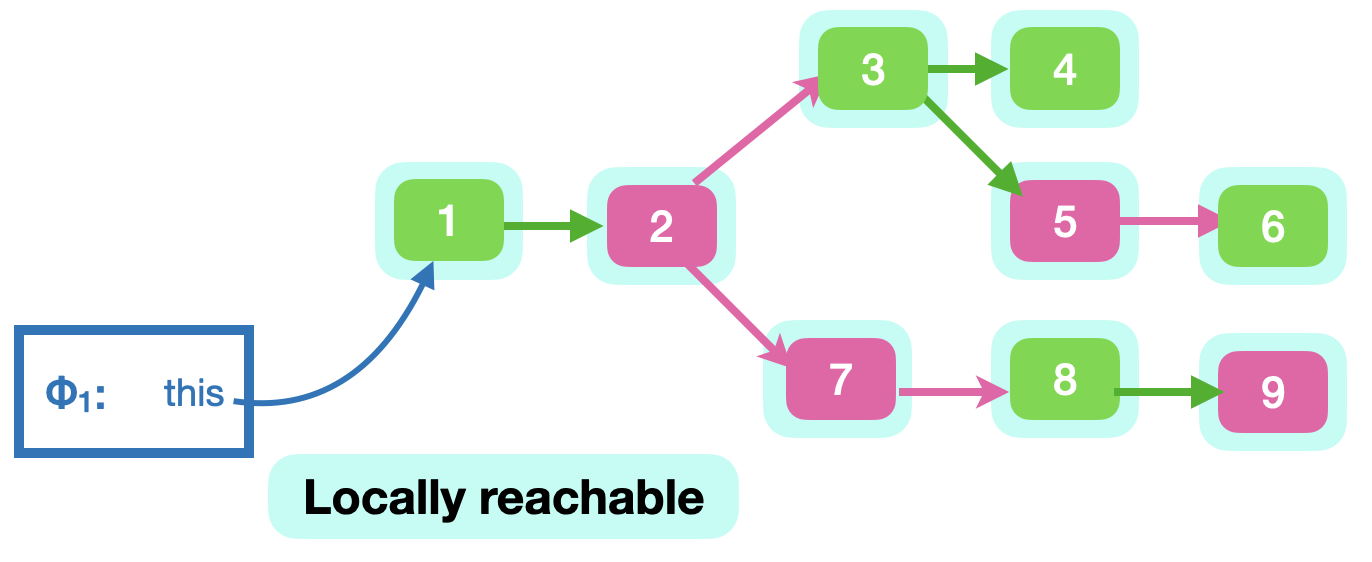
\includegraphics[width=\linewidth]{diagrams/locReachA.png}
} 
&
\resizebox{5cm}{!}{
\includegraphics[width=\linewidth]{diagrams//locReachb.png}
} 
\\
\hline
 a heap
&
Locally Reachable from $\phi_1$
&
Locally Reachable from $\phi_2$
\\
\hline \hline
\end{tabular}
   \caption{A heap, and locally Reachable Objects from $\phi_1$ and $\phi_2$ }
   \label{fig:LReachable}
 \end{figure}

We illustrate these concepts in Fig. \ref{fig:LReachable}: In the middle pane the top frame is $\phi_1$ which maps \prg{this} to $o_1$; all objects are locally reachable. 
In the right pane the top frame is $\phi_2$, which maps \prg{this} to $o_3$, and $x$ to $o_7$; now $o_1$ and $o_2$ are no longer locally reachable.

Lemma  \ref{lemma:relevant} % describes properties of global reachability. 
says that  (\ref{oneGR}) Locally reachable objects are globally reachable, and 
(\ref{twoGR}) Any object which will be globally reachable at some future state  and which exists object in the current state, is globally reachable the current state: that is, 
a globally unreachable object may not become reachable in the future.
\footnoteSD{cite "only connectivity begets connectivity"}
%\sdN{(3) the objects locally reachable after a method call were also locally reachable before the call.}
%; the requirement in the premise  that the arguments of the call, $\overline o$, are locally reachable is not a restriction, because, by construction, the arguments to a method call are locally reachable.}
%Lemma \ref{lemma:relevant:after:bounded} describes properties of local reachability. It is 
%is the counterpart to lemma \ref{lemma:relevant} --  with the difference that   part  \ref{threeLR} hasthe  stronger  premise that they  requires bounded executions. In more detail (\ref{oneLR}) a locally reachable of object after a method call 
%was locally reachable before the call. (\ref{twoLR}) Bounded execution cannot turn an unreachable object to globally reachable. (\ref{tthreeLR}) Bounded execution cannot 



\begin{lemma}
\label{lemma:relevant}
For all module sets $\Mtwo$, states $\sigma$, $\sigma'$, $\sigma''$ for all objects $o$, $\overline o$, atoms ${\overline \va}:$\footnoteSD{\sdN{TODO decide whether $o$ or $\alpha$}}
%and  variables ${\overline z}$, and statements $s:$
\begin{enumerate}
\item
\label{oneGR}
$ \LRelevant \alpha \sigma\ \ \Longrightarrow \ \   \GRelevant \alpha \sigma$
\item
\label{twoGR}
$\GRelevant o {\sigma'}  \ \wedge\ \ \leadstoBoundedStar  {\Mtwo}   \sigma  {\sigma}  {\sigma'} \ \wedge \ \sdN{o\in \sigma} \ \ \Longrightarrow \ \  \GRelevant o {\sigma}$
%\end{enumerate}
%\end{lemma}
 %% \subsubsection{{Reachable  Objects and Bounded Execution}}
%\begin{lemma}
%\label{lemma:relevant:after:bounded}
%{For all states $\sigma$, $\sigma'$, and $\sigma''$,for all objects $o$, and for all modules  $M$:
%\begin{enumerate}
\item
\label{threeGR}
${\leadstoBoundedStar {\Mtwo}  {\sigma} {\sigma''} {\sigma'}} \ \ \wedge \ \  \GRelevant o {\sigma'} \ \ \wedge\ \  \sdN{o\in \sigma} \ \ \ \Longrightarrow \ \  \ \GRelevant o {\sigma}$.
\item
\label{oneLR}
\sdN{$\sigma'\in \PushS {o} {\sigma}  \ \ \wedge \ \  \LRelevant {\overline o} {\sigma} \ \ \wedge\ \   \LRelevant o {\sigma'} \ \ \ \Longrightarrow \ \ \  \LRelevant o {\sigma}$
}
\item
\label{threeLR}
${\leadstoBoundedStar {\Mtwo}  {\sigma}  {\sigma} {\sigma'}} \ \ \wedge \ \   \LRelevant o {\sigma'}\  \ \wedge\ \  \sdN{o\in \sigma} \ \ \ \Longrightarrow \ \ \ \LRelevant o {\sigma}$.
\end{enumerate}
\end{lemma}

\sdN{Consider Fig.  \ref{fig:UpSemantics}, the lemma above promises that any objects locally reachable in $\sigma_{14}$ which already existed in $\sigma_{8}$, were locally accessible in $\sigma_{8}$. However, the lemma is only  applicable to bounded execution, and as 
$\notLeadstoBoundedStar {\Mtwo} {\sigma_8} {\sigma_8} {\sigma_{17}}$, 
the lemma does not promise that  objects locally reachable in $\sigma_{17}$ which already existed in $\sigma_{8}$, were locally accessible in $\sigma_{8}$ -- namely it could be hat object are made globally reachable during the step from $\sigma_{15}$ to $\sigma_{16}$.}








